%This file was automatically generated by [prove].

\title{Graph}
\documentclass[landscape, 11pt]{article}

\usepackage{tikz}
\usetikzlibrary{calc}
\usetikzlibrary{positioning}
\usetikzlibrary{arrows.meta}

\usepackage[margin=0pt, hoffset=0pt, voffset=0pt, top=20pt,bottom=20pt]{geometry}

\usepackage{color}
\definecolor{inactive}{rgb}{0.9, 0.9, 0.9}
\definecolor{darkmagenta}{rgb}{0.55, 0.0, 0.55}
\definecolor{darkorange}{rgb}{1.0, 0.55, 0.0}
\definecolor{darkpastelgreen}{rgb}{0.01, 0.75, 0.24}
\definecolor{oucrimsonred}{rgb}{0.6, 0.0, 0.0}
\definecolor{darkpowderblue}{rgb}{0.0, 0.2, 0.6}
\definecolor{mediumspringgreen}{rgb}{0.0, 0.98, 0.6}
\definecolor{deepskyblue}{rgb}{0.0, 0.75, 1.0}
\definecolor{brightpink}{rgb}{1.0, 0.0, 0.5}

\usepackage{calc}
\usepackage{subcaption}
\newsavebox\tlegend
\newlength\tlegendheight
\newsavebox\tgraph

\usepackage{listings}
\newlength\tgraphheight

\pagenumbering{gobble}


\begin{document}

%Legend
\sbox{\tlegend}{
\resizebox{0.9\hsize}{!}{
\begin{tikzpicture}[node distance = 1pt, auto]
\node (IMPL) at (0pt,0pt) {\texttt{IMPL}: node is part of an implication};
\node[right = 30pt of IMPL] (EQTY){\texttt{EQTY}: node is part of an equality};
\node[right = 30pt of EQTY] (FMLA){\texttt{FMLA}: node is part of an ordinary formula};
\node[right = 30pt of FMLA] (ASMP){\texttt{ASMP}: node is an assumption};
\node[right = 30pt of ASMP] (NEWC){\texttt{NEWC}: node contains a newly introduced constant};
\node[right = 30pt of NEWC] (LOCK){\texttt{LOCK}: \texttt{ASMP} flag is locked for the entire subtree};
\node[right = 30pt of LOCK] (FRST){\texttt{FRST}: node is positioned before first occurrence of an implication formulator in that formula};
\node[right = 30pt of FRST] (TRUE){statement is true};
\node[right = 30pt of TRUE] (VAR){subtree contains at least one variable};
\draw[-{Triangle[length=10pt,width=10pt]}, color=darkmagenta] ([xshift=-10pt] IMPL.west)to (IMPL.west);
\draw[-{Triangle[length=10pt,width=10pt]}, color=darkorange] ([xshift=-10pt] EQTY.west)to (EQTY.west);
\draw[-{Triangle[length=10pt,width=10pt]}, color=darkpastelgreen] ([xshift=-10pt] FMLA.west)to (FMLA.west);
\draw[-{Triangle[length=10pt,width=10pt]}, color=oucrimsonred] ([xshift=-10pt] ASMP.west)to (ASMP.west);
\draw[-{Triangle[length=10pt,width=10pt]}, color=darkpowderblue] ([xshift=-10pt] NEWC.west)to (NEWC.west);
\draw[-{Triangle[length=10pt,width=10pt]}, color=mediumspringgreen] ([xshift=-10pt] LOCK.west)to (LOCK.west);
\draw[-{Triangle[length=10pt,width=10pt]}, color=deepskyblue] ([xshift=-10pt] FRST.west)to (FRST.west);
\draw[-{Triangle[length=10pt,width=10pt]}, color=brightpink] ([xshift=-10pt] TRUE.west)to (TRUE.west);
\draw[-{Triangle[length=10pt,width=10pt]}, color=black] ([xshift=-10pt] VAR.west)to (VAR.west);
\end{tikzpicture} } }
\sbox{\tgraph}{
\resizebox{0.9\hsize}{!}{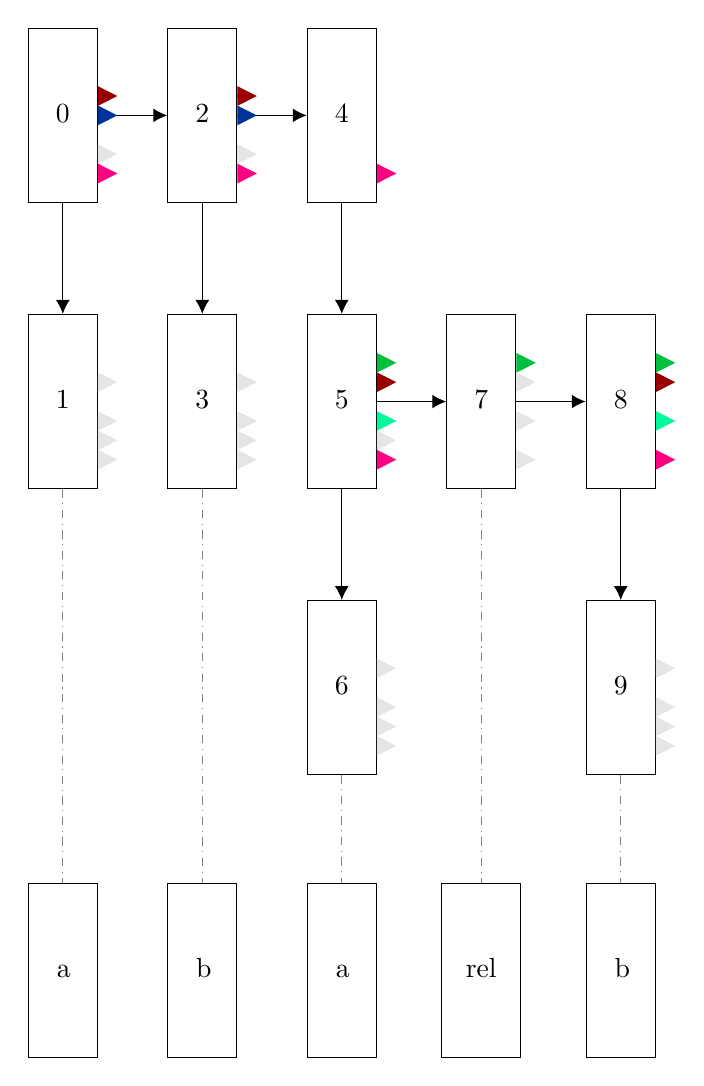
\begin{tikzpicture}[node distance = 1pt, auto]

%nodes and arrows numbered in pre-order traversal
\begin{scope}[every node/.style={rectangle,inner sep=3pt,minimum width=25pt, minimum height=63pt, text height=5pt,yshift=0pt}, -{Latex[length=5pt,width=5pt]}]

\node[draw] (0) at (0pt,0pt) {$0$};
\node[draw, below = 40pt of 0] (1) {$1$};
\draw (0.south) -- (1.north);
\node[draw, right = 25pt] (2) at (0 -| 1.east) {\textrm{2}};
\draw (0.east) -- (2.west);
\node[draw, below = 40pt of 2] (3) {$3$};
\draw (2.south) -- (3.north);
\node[draw, right = 25pt] (4) at (2 -| 3.east) {\textrm{4}};
\draw (2.east) -- (4.west);
\node[draw, below = 40pt of 4] (5) {$5$};
\draw (4.south) -- (5.north);
\node[draw, below = 40pt of 5] (6) {$6$};
\draw (5.south) -- (6.north);
\node[draw, right = 25pt] (7) at (5 -| 6.east) {\textrm{7}};
\draw (5.east) -- (7.west);
\node[draw, right = 25pt of 7] (8)  {$8$};
\draw (7.east) -- (8.west);
\node[draw, below = 40pt of 8] (9) {$9$};
\draw (8.south) -- (9.north);

\end{scope}


%symbols corresponding to nodes, read before freeing memory of the graph
\begin{scope}[every node/.style={rectangle,inner sep=3pt,minimum width=25pt, minimum height=63pt, text height=5pt,yshift=0pt}, -]
\node (symalign) at (0pt,-309pt) {};

\draw[-{Triangle[length=7pt,width=7pt]}, color=inactive] ([yshift=7.0pt] 9.east) to ([yshift=7.0pt, xshift=7pt] 9.east);
\draw[-{Triangle[length=7pt,width=7pt]}, color=inactive] ([yshift=-7.0pt] 9.east) to ([yshift=-7.0pt, xshift=7pt] 9.east);
\draw[-{Triangle[length=7pt,width=7pt]}, color=inactive] ([yshift=-14.0pt] 9.east) to ([yshift=-14.0pt, xshift=7pt] 9.east);
\draw[-{Triangle[length=7pt,width=7pt]}, color=inactive] ([yshift=-21.0pt] 9.east) to ([yshift=-21.0pt, xshift=7pt] 9.east);
\node[draw] (s9) at (symalign -| 9) {\lstinline| b |};
\draw[thin, dash dot, color=gray] (9.south) -- (s9.north);
\draw[-{Triangle[length=7pt,width=7pt]}, color=darkpastelgreen] ([yshift=14.0pt] 8.east) to ([yshift=14.0pt, xshift=7pt] 8.east);
\draw[-{Triangle[length=7pt,width=7pt]}, color=oucrimsonred] ([yshift=7.0pt] 8.east) to ([yshift=7.0pt, xshift=7pt] 8.east);
\draw[-{Triangle[length=7pt,width=7pt]}, color=mediumspringgreen] ([yshift=-7.0pt] 8.east) to ([yshift=-7.0pt, xshift=7pt] 8.east);
\draw[-{Triangle[length=7pt,width=7pt]}, color=brightpink] ([yshift=-21.0pt] 8.east) to ([yshift=-21.0pt, xshift=7pt] 8.east);
\draw[-{Triangle[length=7pt,width=7pt]}, color=darkpastelgreen] ([yshift=14.0pt] 7.east) to ([yshift=14.0pt, xshift=7pt] 7.east);
\draw[-{Triangle[length=7pt,width=7pt]}, color=inactive] ([yshift=7.0pt] 7.east) to ([yshift=7.0pt, xshift=7pt] 7.east);
\draw[-{Triangle[length=7pt,width=7pt]}, color=inactive] ([yshift=-7.0pt] 7.east) to ([yshift=-7.0pt, xshift=7pt] 7.east);
\draw[-{Triangle[length=7pt,width=7pt]}, color=inactive] ([yshift=-21.0pt] 7.east) to ([yshift=-21.0pt, xshift=7pt] 7.east);
\node[draw] (s7) at (symalign -| 7) {\lstinline| rel |};
\draw[thin, dash dot, color=gray] (7.south) -- (s7.north);
\draw[-{Triangle[length=7pt,width=7pt]}, color=inactive] ([yshift=7.0pt] 6.east) to ([yshift=7.0pt, xshift=7pt] 6.east);
\draw[-{Triangle[length=7pt,width=7pt]}, color=inactive] ([yshift=-7.0pt] 6.east) to ([yshift=-7.0pt, xshift=7pt] 6.east);
\draw[-{Triangle[length=7pt,width=7pt]}, color=inactive] ([yshift=-14.0pt] 6.east) to ([yshift=-14.0pt, xshift=7pt] 6.east);
\draw[-{Triangle[length=7pt,width=7pt]}, color=inactive] ([yshift=-21.0pt] 6.east) to ([yshift=-21.0pt, xshift=7pt] 6.east);
\node[draw] (s6) at (symalign -| 6) {\lstinline| a |};
\draw[thin, dash dot, color=gray] (6.south) -- (s6.north);
\draw[-{Triangle[length=7pt,width=7pt]}, color=darkpastelgreen] ([yshift=14.0pt] 5.east) to ([yshift=14.0pt, xshift=7pt] 5.east);
\draw[-{Triangle[length=7pt,width=7pt]}, color=oucrimsonred] ([yshift=7.0pt] 5.east) to ([yshift=7.0pt, xshift=7pt] 5.east);
\draw[-{Triangle[length=7pt,width=7pt]}, color=mediumspringgreen] ([yshift=-7.0pt] 5.east) to ([yshift=-7.0pt, xshift=7pt] 5.east);
\draw[-{Triangle[length=7pt,width=7pt]}, color=inactive] ([yshift=-14.0pt] 5.east) to ([yshift=-14.0pt, xshift=7pt] 5.east);
\draw[-{Triangle[length=7pt,width=7pt]}, color=brightpink] ([yshift=-21.0pt] 5.east) to ([yshift=-21.0pt, xshift=7pt] 5.east);
\draw[-{Triangle[length=7pt,width=7pt]}, color=brightpink] ([yshift=-21.0pt] 4.east) to ([yshift=-21.0pt, xshift=7pt] 4.east);
\draw[-{Triangle[length=7pt,width=7pt]}, color=inactive] ([yshift=7.0pt] 3.east) to ([yshift=7.0pt, xshift=7pt] 3.east);
\draw[-{Triangle[length=7pt,width=7pt]}, color=inactive] ([yshift=-7.0pt] 3.east) to ([yshift=-7.0pt, xshift=7pt] 3.east);
\draw[-{Triangle[length=7pt,width=7pt]}, color=inactive] ([yshift=-14.0pt] 3.east) to ([yshift=-14.0pt, xshift=7pt] 3.east);
\draw[-{Triangle[length=7pt,width=7pt]}, color=inactive] ([yshift=-21.0pt] 3.east) to ([yshift=-21.0pt, xshift=7pt] 3.east);
\node[draw] (s3) at (symalign -| 3) {\lstinline| b |};
\draw[thin, dash dot, color=gray] (3.south) -- (s3.north);
\draw[-{Triangle[length=7pt,width=7pt]}, color=oucrimsonred] ([yshift=7.0pt] 2.east) to ([yshift=7.0pt, xshift=7pt] 2.east);
\draw[-{Triangle[length=7pt,width=7pt]}, color=darkpowderblue] ([yshift=0.0pt] 2.east) to ([yshift=0.0pt, xshift=7pt] 2.east);
\draw[-{Triangle[length=7pt,width=7pt]}, color=inactive] ([yshift=-14.0pt] 2.east) to ([yshift=-14.0pt, xshift=7pt] 2.east);
\draw[-{Triangle[length=7pt,width=7pt]}, color=brightpink] ([yshift=-21.0pt] 2.east) to ([yshift=-21.0pt, xshift=7pt] 2.east);
\draw[-{Triangle[length=7pt,width=7pt]}, color=inactive] ([yshift=7.0pt] 1.east) to ([yshift=7.0pt, xshift=7pt] 1.east);
\draw[-{Triangle[length=7pt,width=7pt]}, color=inactive] ([yshift=-7.0pt] 1.east) to ([yshift=-7.0pt, xshift=7pt] 1.east);
\draw[-{Triangle[length=7pt,width=7pt]}, color=inactive] ([yshift=-14.0pt] 1.east) to ([yshift=-14.0pt, xshift=7pt] 1.east);
\draw[-{Triangle[length=7pt,width=7pt]}, color=inactive] ([yshift=-21.0pt] 1.east) to ([yshift=-21.0pt, xshift=7pt] 1.east);
\node[draw] (s1) at (symalign -| 1) {\lstinline| a |};
\draw[thin, dash dot, color=gray] (1.south) -- (s1.north);
\draw[-{Triangle[length=7pt,width=7pt]}, color=oucrimsonred] ([yshift=7.0pt] 0.east) to ([yshift=7.0pt, xshift=7pt] 0.east);
\draw[-{Triangle[length=7pt,width=7pt]}, color=darkpowderblue] ([yshift=0.0pt] 0.east) to ([yshift=0.0pt, xshift=7pt] 0.east);
\draw[-{Triangle[length=7pt,width=7pt]}, color=inactive] ([yshift=-14.0pt] 0.east) to ([yshift=-14.0pt, xshift=7pt] 0.east);
\draw[-{Triangle[length=7pt,width=7pt]}, color=brightpink] ([yshift=-21.0pt] 0.east) to ([yshift=-21.0pt, xshift=7pt] 0.east);

\end{scope}

\end{tikzpicture} } }

\begin{figure}[h!]\centering
%\begin{subfigure}{\textwidth}\centering\usebox{\tlegend}\end{subfigure}\vspace{10pt}
\begin{subfigure}{\textwidth}\centering\usebox{\tgraph}\end{subfigure}
\end{figure}

%\settototalheight\tlegendheight{\usebox{\tlegend}}
\settototalheight\tgraphheight{\usebox{\tgraph}}
%\addtolength{\tgraphheight}{\tlegendheight}
\addtolength{\tgraphheight}{50pt}
\pdfpageheight=\the\tgraphheight
\end{document}